% -*- coding: utf-8 -*-
\documentclass[12pt,a4paper]{article}

% поддержка русского
\usepackage[T2A]{fontenc}
\usepackage[utf8]{inputenc}
\usepackage[russian]{babel}
\usepackage{cmap}            % копирование кириллицы из PDF

% математические пакеты
\usepackage{amsmath,amssymb}
\usepackage[fleqn]{amsmath}  % выравнивание формул слева

% графика
\usepackage{graphicx}
% Все изображения лежат в каталоге Graphics
\graphicspath{{Graphics/}}

% гиперссылки
\usepackage[hidelinks]{hyperref}

% отступы
\setlength{\parindent}{1em}
\setlength{\parskip}{0.5em}

% заголовок
\title{Отчет по части I}
\date{}

\begin{document}
\maketitle

\section*{Отчет Аскара}
%--------------------------------------------------
\section*{Часть 1. Зависимость от параметров распределений}
\vspace{-1em}
\noindent
Значения на графиках — это среднее по $M=100$ независимым реализациям для каждого набора параметров. Число вершин графа $n=100$, параметр $k=5$ для kNN-графа и порог $d=1$ для DIST-графа.

\begin{enumerate}
  \item \textbf{kNN-граф:} Среднее число компонент связности практически не зависит от параметра $\alpha$ SkewNormal (почти горизонтальная кривая около $6$–$6.5$). Для Student-t с ростом $\nu$ число компонент убывает, то есть при «тяжёлых хвостах» ($\nu$ — меньше) граф рассоединён сильнее.

  \item \textbf{DIST-граф:} Среднее кликовое число минимально при $\alpha=0$ и симметрично растёт при удалении от нуля (от $\sim40$ до $\sim70$). Для Student-t кликовое число увеличивается с $\nu$ (от $\sim30$ при $\nu\approx1$ до $\sim40$–$45$ при $\nu\approx10$).
\end{enumerate}

\begin{center}
  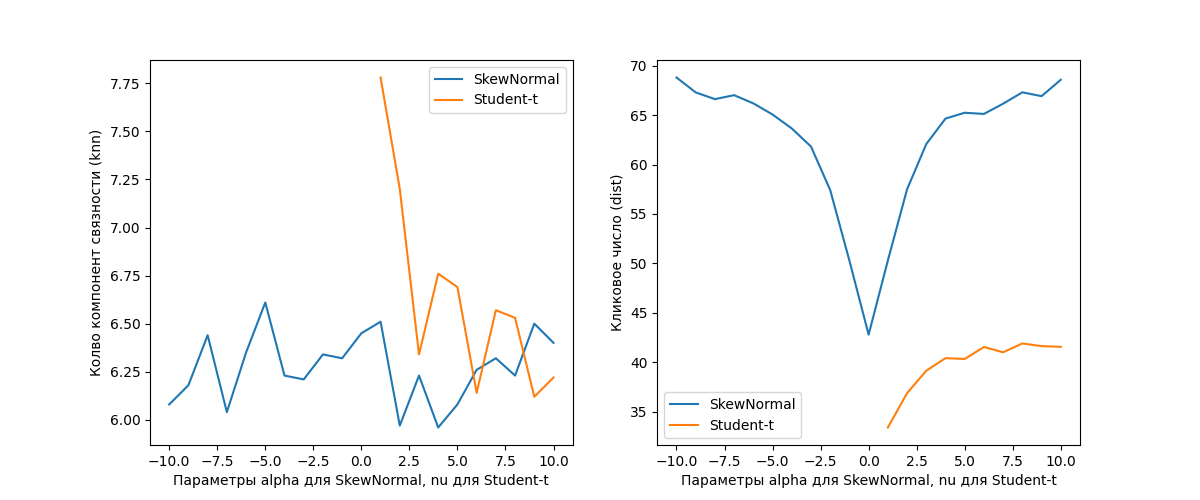
\includegraphics[width=0.9\linewidth]{part1_results_Askar.png}
\end{center}

\newpage
\section*{Часть 2. Зависимость от $n$, $k$ и $d$}
\vspace{-1em}
\noindent
Значения на графиках — это среднее по $M=100$ независимым реализациям для каждого набора параметров.

\begin{itemize}
  \item \textbf{kNN-граф:}
    \begin{itemize}
      \item При увеличении числа вершин $n$ (при $\alpha=\alpha_0$, $\nu=\nu_0$, $k=5$) среднее число компонент связности возрастает.
      \item При увеличении числа соседей $k$ (при $\alpha=\alpha_0$, $\nu=\nu_0$, $n=100$) число компонент резко убывает.
    \end{itemize}

  \item \textbf{DIST-граф:}
    \begin{itemize}
      \item При увеличении числа вершин $n$ (при $\alpha=\alpha_0$, $\nu=\nu_0$, $d=1$) среднее кликовое число растёт, причём скорость роста выше для SkewNormal-графов.
      \item При увеличении $d$ (при $\alpha=\alpha_0$, $\nu=\nu_0$, $n=100$) кликовое число также увеличивается, и для SkewNormal-графов этот рост быстрее. Рост вызван тем, что точки чаще попадают в радиус $d$.
    \end{itemize}
\end{itemize}

\begin{center}
  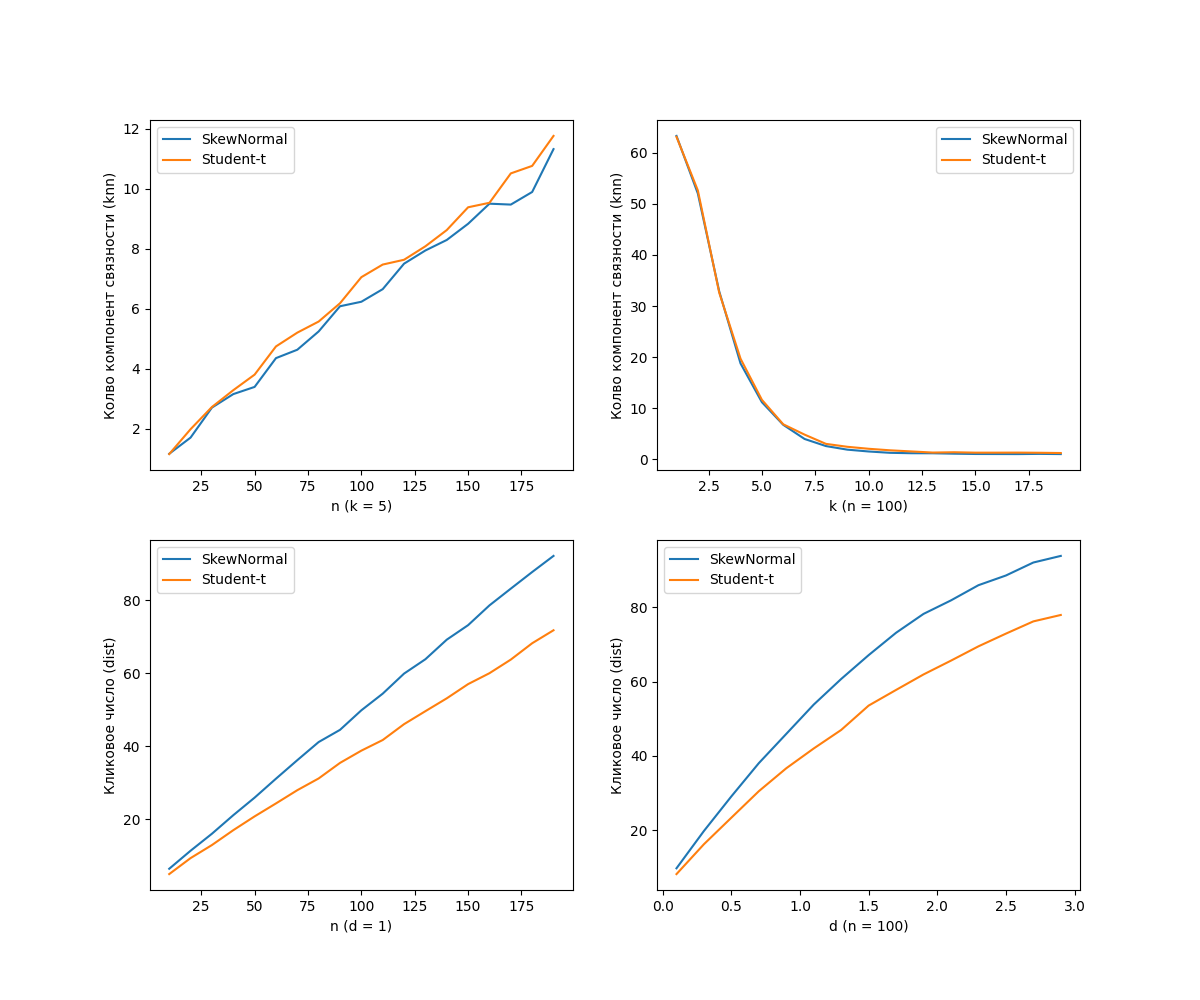
\includegraphics[width=0.9\linewidth]{part2_results_Askar.png}
\end{center}

\section*{Часть 3. Разделяющая способность статистик}
\vspace{-1em}
\noindent
Построено по $M_{\text{large}}=5000$ реализаций каждого распределения.

\begin{center}
  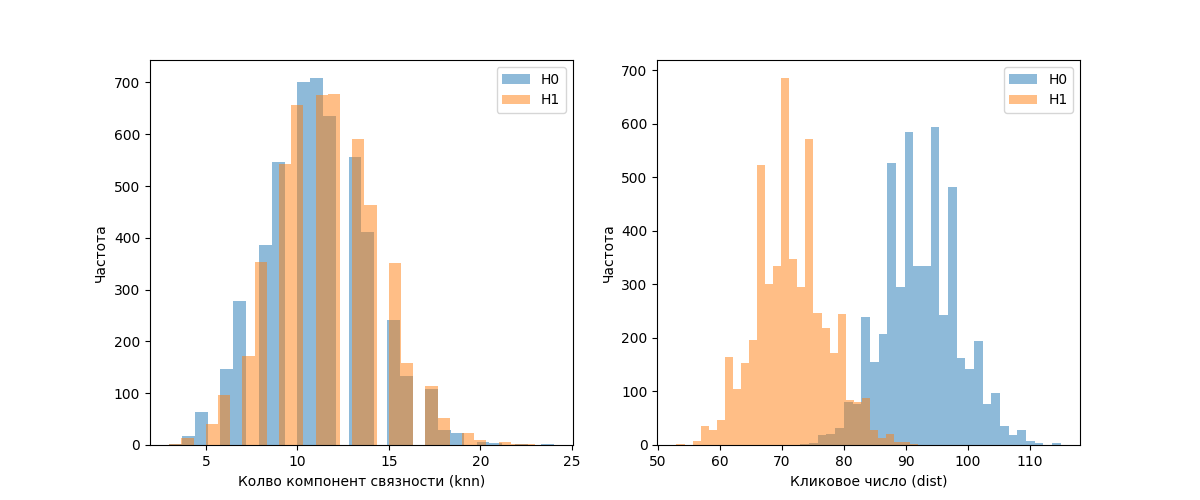
\includegraphics[width=0.8\linewidth]{part3_results_0_Askar.png}
\end{center}
\begin{center}
  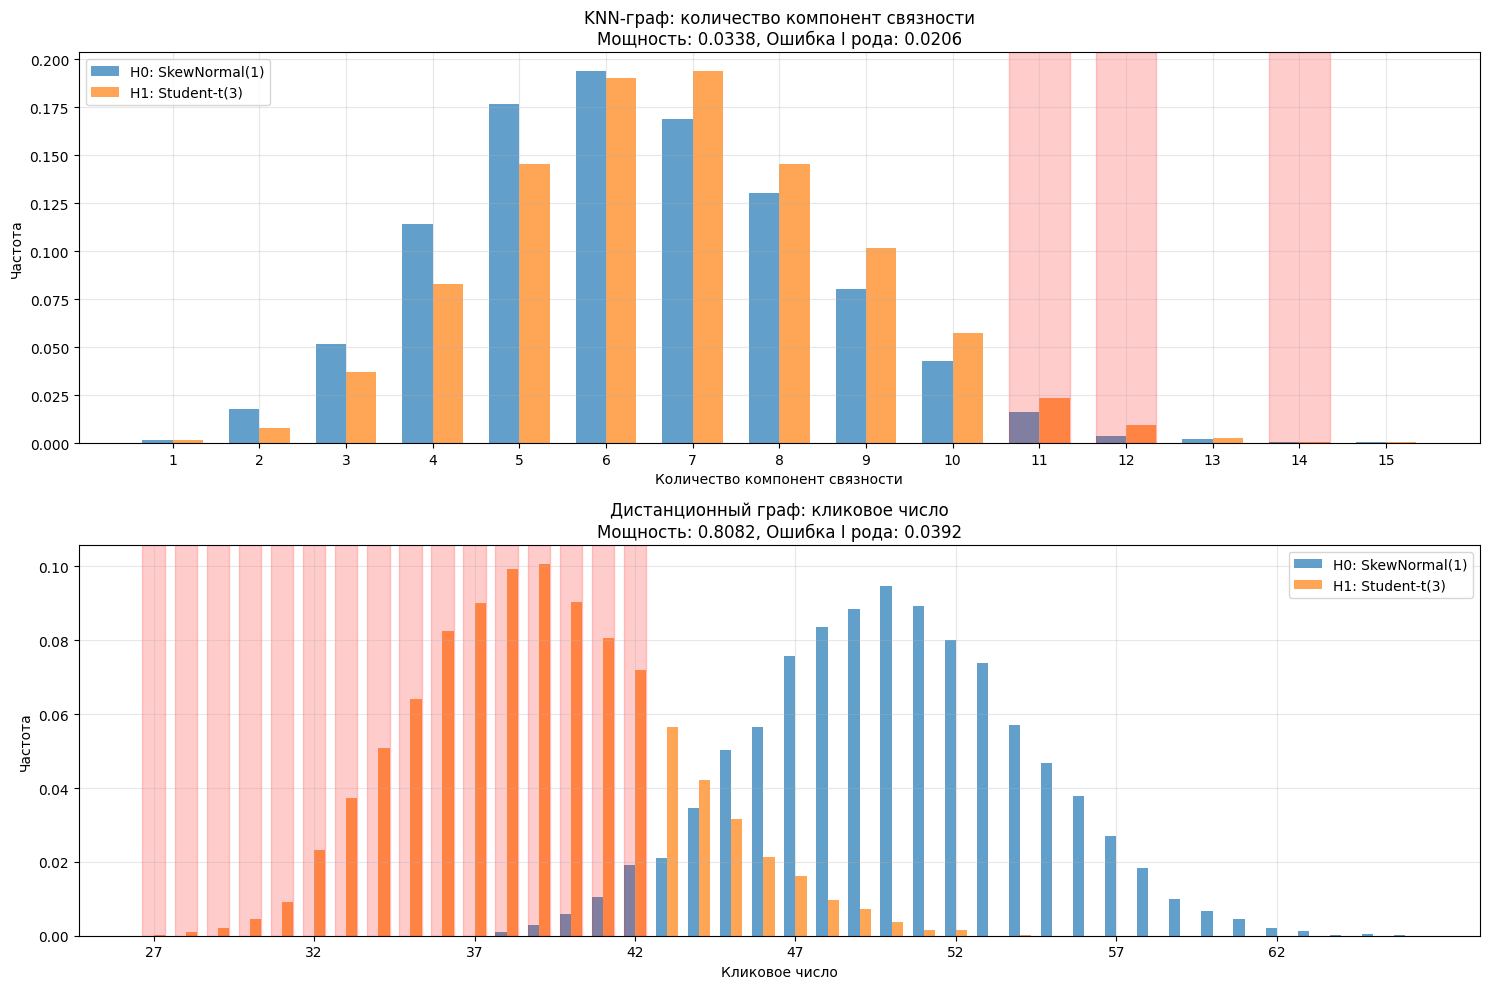
\includegraphics[width=\linewidth]{part3_results_1_Askar.png}
\end{center}

\begin{itemize}
  \item \textbf{kNN-граф:} Распределения числа компонент при $H_0$ и $H_1$ сильно перекрываются — низкая разделяющая способность, мощность маленькая.
  \item \textbf{DIST-граф:} Распределения кликового числа сдвинуты друг от друга: для SkewNormal значения пик около 50, для Student-t — около 39. Красная зона — область принятия $H_1$: мощность выше.
\end{itemize}

% ===================== ДОБАВЛЕНО: ОТЧЕТ ЯРОСЛАВА =====================

\newpage
\section*{Отчет Ярослава}
\addcontentsline{toc}{section}{Отчет Ярослава}

\subsection*{Часть 1. Влияние параметров распределений}
\vspace{-1em}
\noindent
Среднее по $M=100$ реализациям, $n=100$, $k=5$ (kNN) / $d=1$ (DIST).

\begin{enumerate}
  \item \textbf{kNN-граф:} Число треугольников почти не меняется при изменении $\lambda$ Weibull (около $150$–$151$); при увеличении дисперсии $\sigma$ у Lognormal падает с $151$ до $91$.
  \item \textbf{DIST-граф:} Кликовое число уменьшилось с $62$ до $27$ при росте $\lambda$ (Weibull) и с $55$ до $50$ при росте $\sigma$ (Lognormal).
\end{enumerate}

\begin{center}
  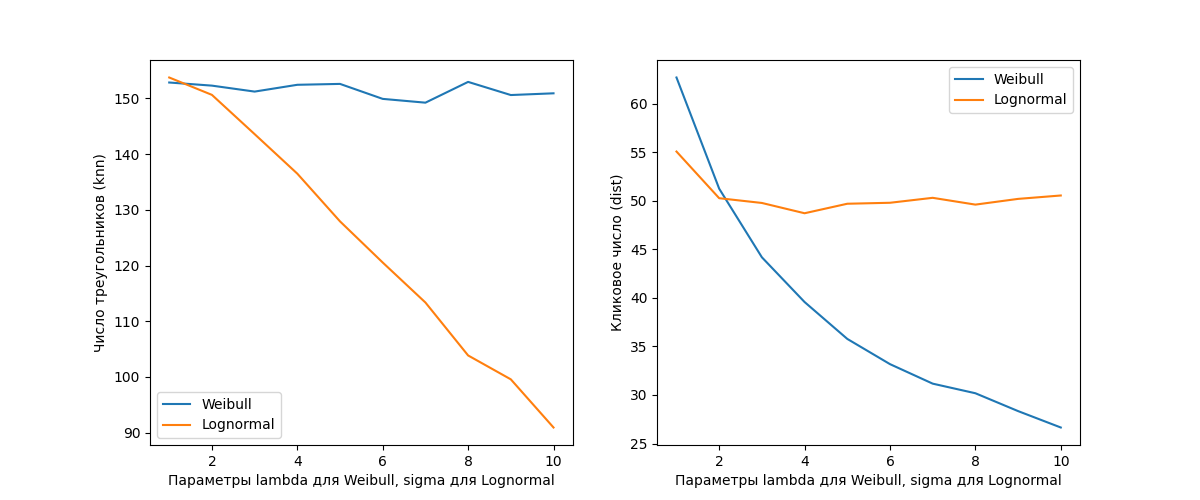
\includegraphics[width=0.9\linewidth]{part1_results_Yaroslav.png}
\end{center}

\subsection*{Часть 2. Зависимость от $n$, $k$ и $d$}
\vspace{-1em}

\begin{center}
  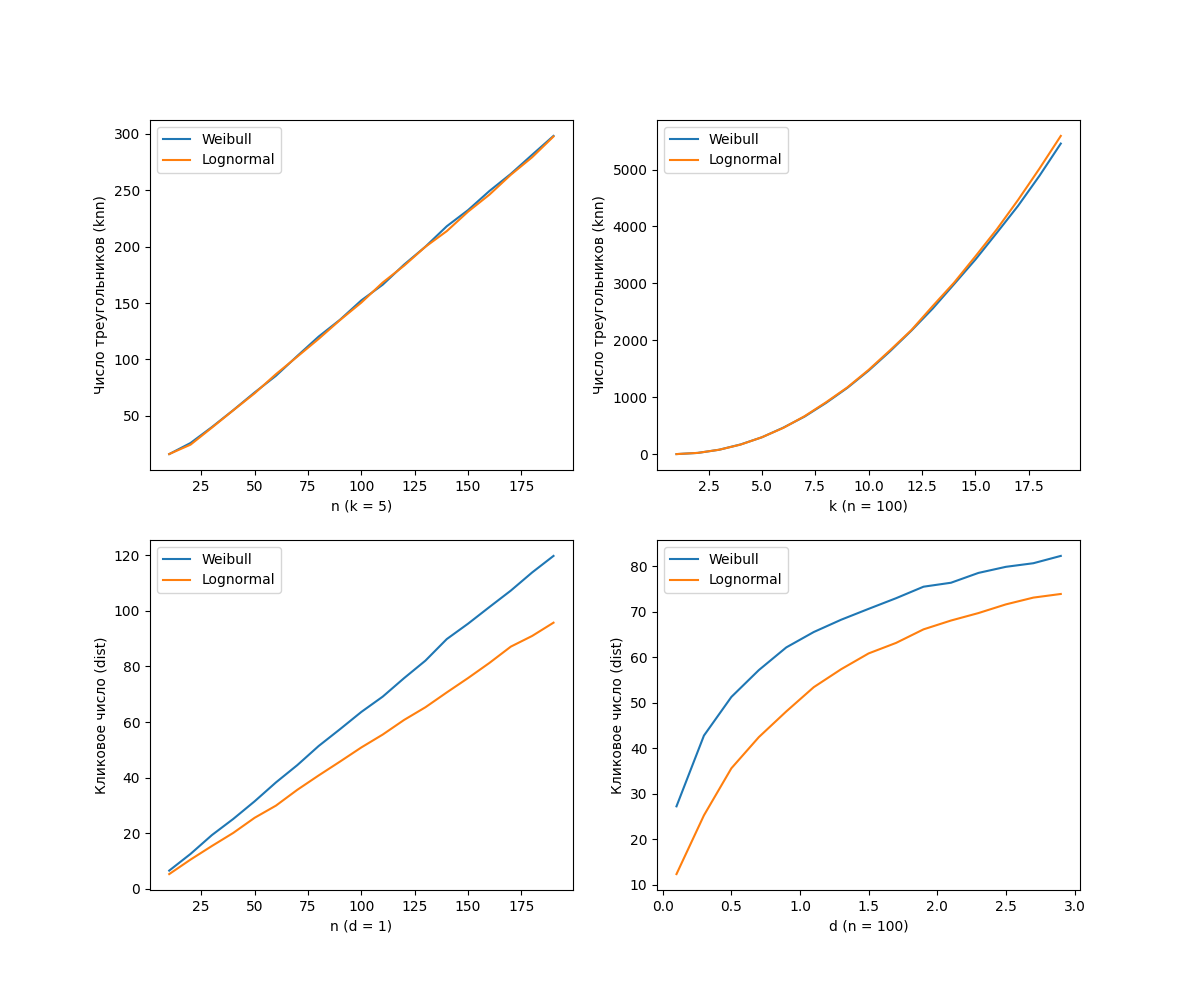
\includegraphics[width=0.9\linewidth]{part2_results_Yaroslav.png}
\end{center}

\subsection*{Выводы}

\begin{enumerate}
  \item Для метрики «треугольники» оба распределения ведут себя почти одинаково --- выбор распределения практически не влияет на~итог.
  \item Для «кликового числа» Weibull формирует более плотные графы: прирост относительно Lognormal усиливается с~ростом~$n$ и~$d$.
  \item Чувствительность метрик:
        \begin{itemize}
          \item «Треугольники» --- сильнее реагируют на~увеличение $k$ (приблизительно $\propto k^{3}$), чем на~$n$ (приблизительно $\propto n$).
          \item «Клики» --- линейны по~$n$, но~по~$d$ быстро достигают плато.
        \end{itemize}
\end{enumerate}

\subsection*{Часть 3. Проверка статистических гипотез}
\vspace{-1em}

\begin{center}
  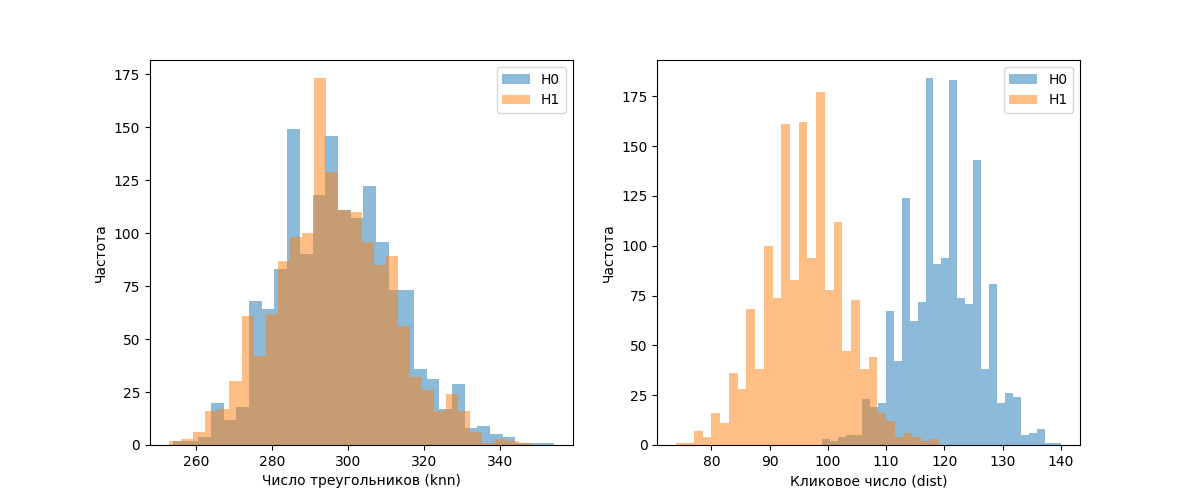
\includegraphics[width=0.8\linewidth]{part3_results_0_Yaroslav.png}
\end{center}
\begin{center}
  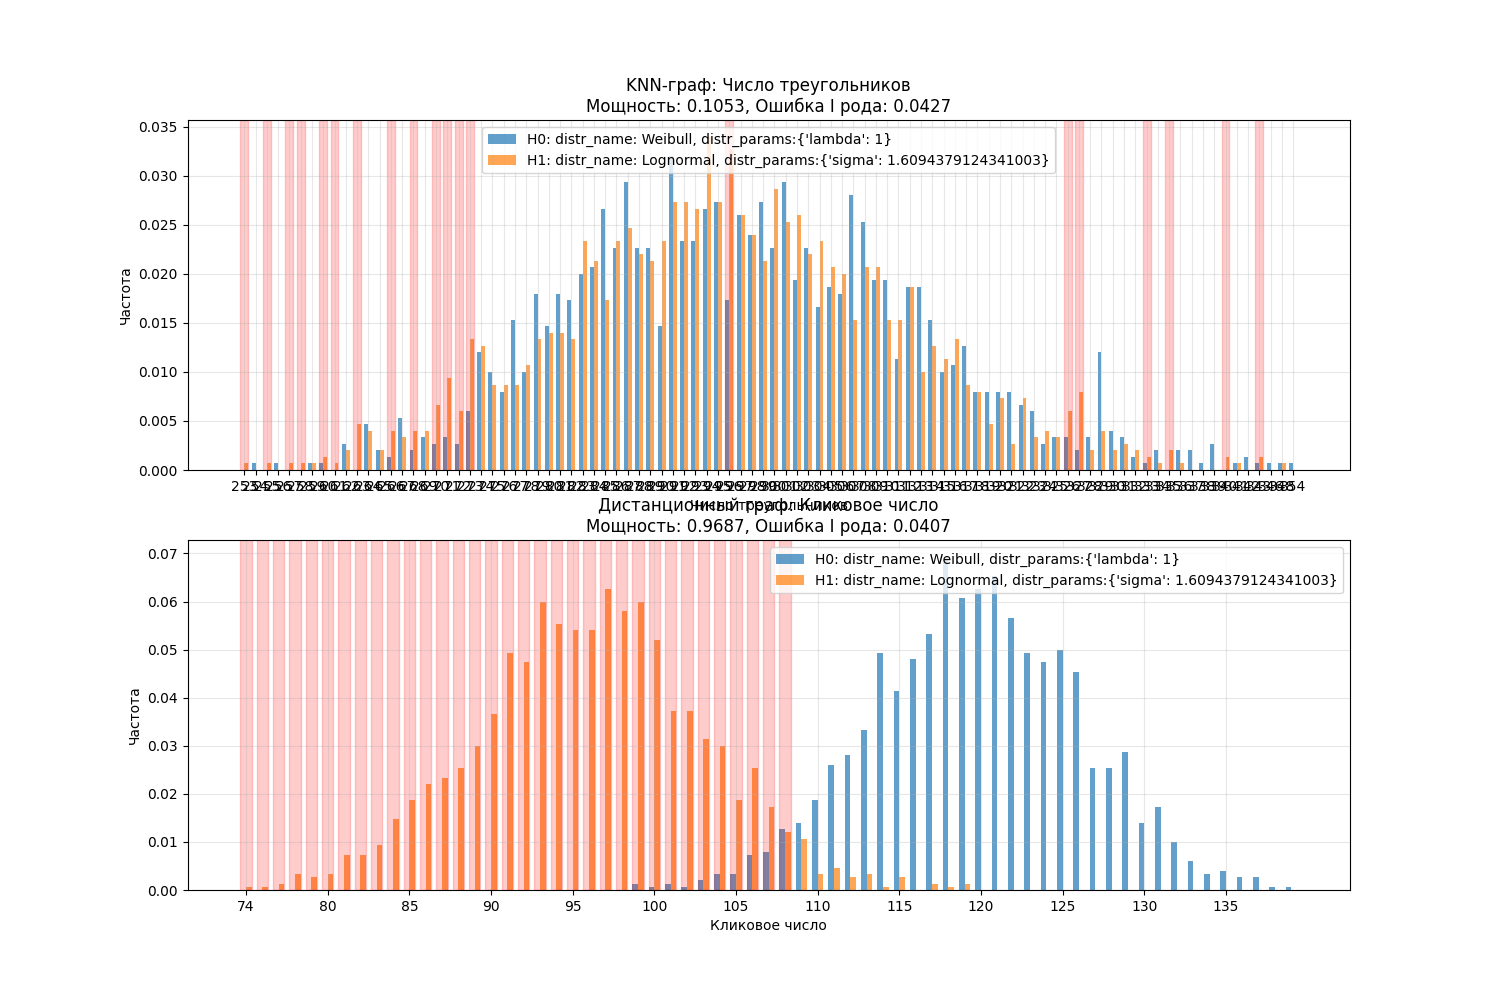
\includegraphics[width=0.95\linewidth]{part3_results_1_Yaroslav.png}
\end{center}

\begin{itemize}
  \item Мощность теста по треугольникам (kNN) составляет $0.1$ при ошибке I рода $0.05$.
  \item Мощность теста по кликовому числу (DIST) — $0.78$ при ошибке $0.03$.
\end{itemize}

% ===================== КОНЕЦ ОТЧЕТА ЯРОСЛАВА =====================

\end{document}
